\chapter{Settimana 1}

\section{Introduzione}

L'obbiettivo della prima settimana è quello di predere confidenza con gli ambienti di lavoro LabVIEW e Matlab e gli strumenti di acquisione.

\vspace{1cm}

\NewDay{Introduzione a LabVIEW}{22/09/2020}

\section{Primo progetto LabVIEW}

\LogMark{Utilizzo controlli e indicatori}{10:30}
Creiamo dei controlli nel "Front Panel" per inserire e visualizzare dei numeri, esplorando le varie impostazioni.
\begin{figure}[H]
\caption{}
    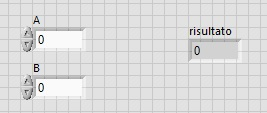
\includegraphics[width=5cm]{settimana_1/immagini/primo_vi.jpg}
    \centering
\end{figure}

\LogMark{Utilizzo BlockDiagram}{10:40}
Utilizziamo la scheda "Block Diagram" di LabView per eseguire i collegamenti ed operazioni base tra i vari controlli precedentemente inseriti
\begin{figure}[H]
\caption{}
    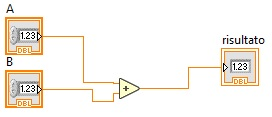
\includegraphics[width=5cm]{settimana_1/immagini/primo_bd.jpg}
    \centering
\end{figure}

\LogMark{Esecuzione del VI creato}{10:55}
Abbiamo eseguito il VI e verificato il corretto funzionamento
\begin{figure}[H]
\caption{}
    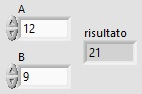
\includegraphics[width=3cm]{settimana_1/immagini/prima_esec.jpg}
    \centering
\end{figure}

\NewSection{Realizzazione di un vettore equispaziato in LabVIEW (Es. 2)}
L'obiettivo dell'esercizio è realizzare un interfacia in LabView (VI) per generare un vettore equispaziato

\LogMark{Utilizzo controlli}{15:06}
Creiamo un ambiente VI in LabVIEW. Inizializzaziamo tre controlli numerici. Infatti per realizzare un vettore necessitiamo di tre parametri, che definiscano univocamente la langhezza e gli estremi del vettore. Adottiamo quali parametri (scelta arbitraria): il valore massimo, il valore minimo e il numero di elementi dell'array. I primi due valori li inizializziamo a double, mentre il terzo a long unsignet int.
Mettiamo quale data entry per i valori massimo e minimo il range $[0, +\infty]$, così da evitare i numeri negativi.
\Nota{L'operazione del data entry è superflua: è stata effettuata solo per prendere mano con l'ambiente di sviluppo}
%A fini esplicativi, introduciamo un indicatore numerico per 

\LogMark{Collegamenti in BlockDiagram}{15:10}
Utilizziamo la scheda "Block Diagram". Realizziamo una differenza del valore massimo rispetto al minimo (guardare la figura \ref{figura:diagramma}). Riduciamo di uno il valore del numero di elementi dell'array. Attuiamo la divisione fra i due risultati così ottenuti. Ne risulta la lunghezza della spaziatura fra due elementi successivi dell'array.
Si realizza un ciclo for. Adottiamo quale numero di passi del ciclo (la cui variabile incremento i parte da 0) il numero di elementi del vettore. All'interno del ciclo, al valore minimo viene sommato $i \cdot \Delta x$, ove $\Delta x$ è la spaziatura fra elementi successivi del vettore.

\LogMark{Utilizzo indicatori e array numerici}{15:17}
Ritorniamo al pannello frontale. Immettiamo un'array e introduciamo al suo interno un indicatore numerico ai fini di esplicarne la funzionalità di output. All'interno del diagramma, all'array vengono quindi assegnati i valori ottenuti in uscita dal ciclo for. 

\LogMark{Realizzazione grafico}{15:30}
Nel pannello frontale introduciamo l'oggetto "waveform graph". All'interno del diagramma, collleghiamo quindi l'uscita del ciclo for al grafico. Il risultato è quello mostrato in figura:
\begin{figure}[H]
\caption{}
    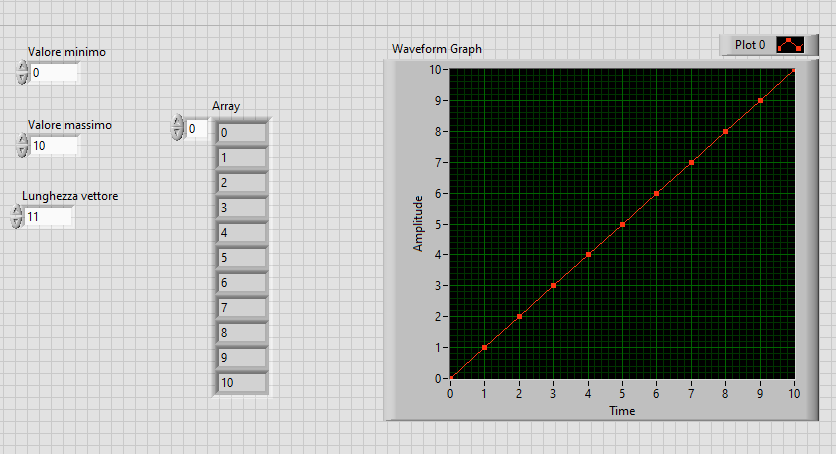
\includegraphics[width=10cm]{settimana_1/immagini/PannelloVettore.png}\label{figura:pannello}
    \centering
\end{figure}

Il "Block Diagramm" corrispondente è:
\begin{figure}[H]
\caption{}
    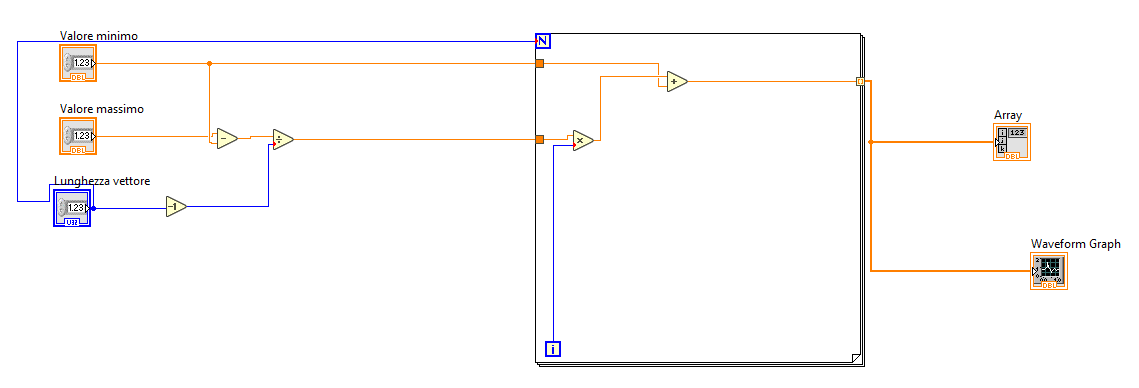
\includegraphics[width=10cm]{settimana_1/immagini/DiagrammVettore.png}
    \label{figura:diagramma}
    \centering
\end{figure}

\Nota{Le caratteristiche di stile ed il tipo di plot effettuato possono essere modificati cliccando l'icona con la forma d'onda sopra il grafico con il tasto destro del mouse. Si apre così un pannello, ove poter selezionare le specifiche desiderate}

\Nota{Se ora salvassimo e poi chiudessimo le finestre di lavoro, alla riapertura i valori in input ritornerebbero azzerati, così come da default nell'inizializzazione. Ond'evitare il mancato salvataggio dei dati, bisogna imporre che i nostri dati siano quelli di default entro il VI di lavoro. Per farlo, nel menù contestuale si deve selezionare \textit{data operations} e la sottovoce \textit{make current value default}}

\LogMark{Utilizzo del VI come nodo}{15:40}
I VI possono essere usati come nodi, ovvero possono essere realizzati per poi essere utilizzati entro altri programmi. Per poter utilizzare un VI come nodo vanno effettuate due operazioni:
\begin{enumerate}
    \item \textbf{realizzare un'icona seria}: l'icona su cui cliccare è quella raffigurante un'oscilloscopio, un'operazionale e due fili, la quale è posizionata in alto a destra del pannello di controllo. Modifico l'icona a piacimento. Questo è il simbolo del nostro oggetto, il quale comparirà ogni qualvolta si utilizza il VI in questione in altri programmi;
    \item \textbf{specificare i canali di input e output}: dopodiché nell'icona a fianco del simbolo realizzato va scelto un frame volto a indicare quanti sono i nostri input (le celle a sinistra) e output (le celle a destra). Una volta scelto il frame opportuno, a ciascuna cella va collegato il rispettivo canale di input/output, così da renderlo visibile a programmi esterni.
\end{enumerate}

Per utilizzare il VI come nodo, creiamo un nuovo progetto ed utilizziamo l'opzione \textit{"Select VI..."} e scegliamo "vettore.vi".

\begin{figure}[H]
\caption{}
    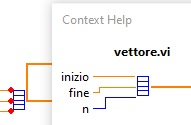
\includegraphics[width=5cm]{settimana_1/immagini/vettore.jpg}
    \centering
\end{figure}

\LogMark{Case nel VI vettore}{16:05}
Utilizziamo l'oggetto \textit{Case Structure} ed un controllo \textit{Push Button} per aggiungere l'opzione per ordinare i valori minimo e massimo in ingresso, collegandoli opportunamente nel \textit{Block Diagram}.

\begin{figure}[H]
\caption{}
    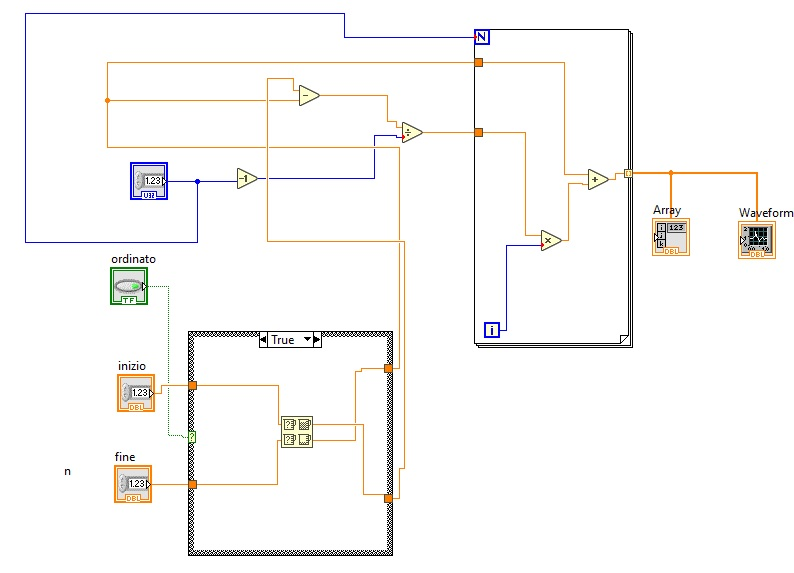
\includegraphics[width=10cm]{settimana_1/immagini/case.jpg}
    \centering
\end{figure}

\NewSection{Grafico carica condensatore (Es. 3-4)}
Vogliamo creare un VI che disegni la funzione modello di carica di un condensatore.

\LogMark{Creazione della funzione modello}{16:40}
Ricordiamo che la carica del condensatore è descritta dall'equazione:
\begin{equation}
    f(t; \tau, A) = A (1 - e^{- {t \over{\tau}}})
\end{equation}
Abbiamo già realizzato un VI per un vettore equispaziato. Di tale ci serviremo per l'array dei tempi t.
Creiamo i controlli numerici necessari a creare l'interfaccia per disegnare la funzione: inizio, fine, tempo caratteristico (chiamato Slide nella figura \ref{figura:diagrammaexp} e $\tau$ nella presente trattazione) e numero di punti disegnati. I primi tre li inizializziamo a double, l'ultimo in unsigned long int. 
Attraverso gli operatori numerici, calcoliamo l'opposto del reciproco della costante tempo $\tau$. Attraverso il diagramma, selezioniamo il VI del vettore realizzato precedentemente e allo stesso passiamo i parametri inizio, fine, N nei canali atti all'input. Dopodiché utilizziamo la funzione $- 1 + e^{- {t \over{\tau}}}$, presente nel modulo \textit{"Functions/Mathematics/Elementary/Exponential"}, per modellizare la nostra equazione. Sempre attraverso gli operatori numerici, invertiamo il nostro risultato di segno. Abbiamo in uscita un array di ordinate per la nostra base dei tempi.

\begin{figure}[H]
\caption{}
    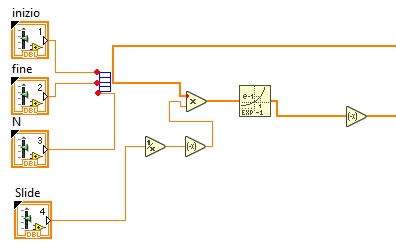
\includegraphics[width=8cm]{settimana_1/immagini/esponenziale.jpg}\label{figura:diagrammaexp}
    \centering
\end{figure}

\LogMark{Grafico della funzione esponenziale}{16:45}
Nel pannello di controllo, introduciamo un \textit{"XY Graph"}, per poter graficare l'array precedentemente calcolato in funzione del vettore che rappresenta la base dei tempi. Questo grafico accetta due vettori, ma solo se combinati in una struttura chiamata cluster. Per costruire un cluster devo inserire un oggetto chiamato bundle (presente in \textit{"Cluster, Class and Variant"}), che ha la funzione di combinare i due array dello stesso tipo in ingresso, fornendo una sola uscita. Il risultato andrà poi collegato al nostro grafico.
Si ottiene così l'andamento desiderato.
\begin{figure}[H]
\caption{}
    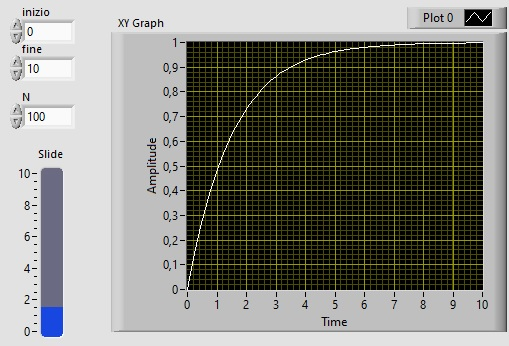
\includegraphics[width=8cm]{settimana_1/immagini/grafico_esponenziale.jpg}
    \centering
\end{figure}

\NewSection{Acquisizione con LabVIEW (Es. 5-8, Hw. 1)}
Vogliamo costruire un semplice VI per controllare l'acquizione di segnali analogici.

\subsection*{Introduzione al MX}
Il MX è l'insieme di tutti i VI che consentono la gestione delle schede di acquisizione. I tre oggetti principali che lo caratterizzano sono:
\begin{itemize}
    \item l'oggetto che imposta il canale;
    \item l'oggetto che stabilisce la tempistica di operazione;
    \item l'oggetto che fa operare il canale.
\end{itemize}

\LogMark{Realizzazione di un VI di acquisizione}{16:55}
Apriamo il diagramma ed il pannello delle funzioni. Inseriamo una funzione Create Channel, presente all'interno della sezione NI DAQmx, a sua volta in Measurement I/O.
Cliccando sulla cella relativa a Create Channel, posso selezionare il tipo di misura che voglio effettuare e che tipo di canale (input/output, analogic/digital, etc.) rappresenta. Volendo vedere dei segnali di tensione generati da un circuito esterno, selezioniamo l'opzione Voltage in  Analog Input.
\sout{Inseriamo un Physical Channel e lo chiamiamo canale. Dopodiché clicchiamo col tasto destro del mouse e selezioniamo Create Control. Nel pannello di controllo, nel controllo relativo a questo canale va inserito il nome del canale in ingresso (al momento non possibile in assenza di una scheda di acquisizione).
Creiamo un controllo}
Cliccando sul canale creato, decidiamo di inserire dei controlli nei seguenti ingressi del canale:
\begin{enumerate}
    \item \textbf{physical channels}: chiamo il relativo controllo \text{"Canale"}. Con questo controllo possiamo selezionare quale canale della scheda adottiamo;
    \item \textbf{input terminal configuration}: possiamo selezionare rispetto a quale linea è riferito il canale (per esemèpio, rispetto alla terra, o rispetto ad un altro canale nella modalità differential, etc.).
\end{enumerate}
Apriamo Pulsante.vi. Al suo interno vi sono tre possibili controlli numerici. Ne copio uno e lo inserisco nel VI di partenza. L'oggetto inserito è un anello (cliccandoci, posso scegliere di fargli assumere uno dei valori discreti tra un numero finito di opzioni predefinite). Il valore che restituisce viene assegnato al maximum value e quello opposto al minimum value. Quindi tramite tale operazione definisco i valori massimo e minimo accettati nella routine. Questa operazione è necessaria ai fini di selezionare un determinato fondo scala per l'acquisizione.
Ora inseriamo un timing (all'interno di NI DAQmx). Cliccandoci, fra le diverse opzioni scegliamo il sample clock. Al task channel in di questo oggetto colleghiamo il task out del Create channel, che vuole usare il riferimento temporale impostato nel timing. Al rate del timing, che regola la frequenza di campionamenti colleghiamo un opportuno controllo rate.
Il prodotto fra la durata complessiva dell'acquisizione e la frequenza di acquisizioni al secondo, convertita in un dato di tipo unsigned long int, mi fornisce il numero totale di campionamenti durante l'acquisizione. Colleghiamo questo risultato al samples per channel del timing.
Inseriamo un controllo al sample mode del timing. Il sample mode mi fornisce delle opzioni sulla modalità di acquisizione dei dati(continuos samples/finite samples/hardware Time Single Point).
Inseriamo un oggetto \text{"read"} (è all'interno di NI DAQmx) e colleghiamo il relativo task in al task out del timing. Il  \text{"read"} fa partire/terminare l'acquisizione a seconda dei segnali rilevati.
Inseriamo uno \text{"stop"} (è all'interno di NI DAQmx) e lo colleghiamo (task in/out al solito) con il \text{"read"}. Lo \text{"stop"} blocca l'uso della risorsa della scheda e la libera.
Inseriamo un grafico di forme d'onda nel pannello di controllo e all'interno del diagramma lo collego al "DAQmx read".
Il pannello frontale ed il "Block Diagramm" realizzati sono riportati di seguito:
\begin{figure}[H]
\caption{}
    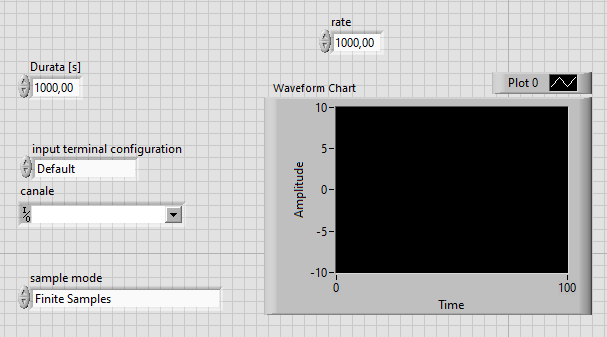
\includegraphics[width=10cm]{settimana_1/immagini/MXACQUISPANEL.png}
    \centering
\end{figure}
\begin{figure}[H]
\caption{}
    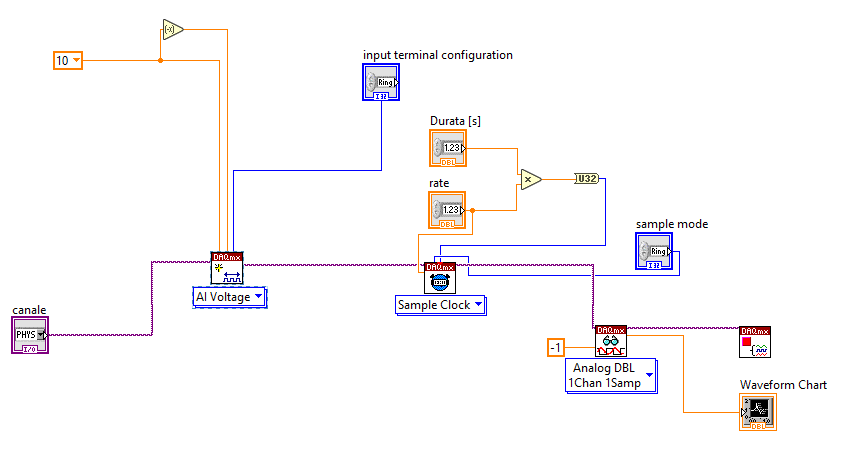
\includegraphics[width=10cm]{settimana_1/immagini/MXACQUISDIAG.png}
    \centering
\end{figure}

%%%%%%%%%%%%%%%%%%%%%%%%%%%%%%%%%%%%%%%%
%%%%%%%%%%%%  NEW DAY %%%%%%%%%%%%%%%%%%
%%%%%%%%%%%%%%%%%%%%%%%%%%%%%%%%%%%%%%%%


\NewDay{Acquisizione dati remota}{24/09/2020}

\NewSection{Acquisizione forme d'onda (Es.9)}

L'obiettivo dell'esercizio è quello di realizzare delle acquisizioni ottimali di forme d'onda.

\LogMark{Acquisizione segnali da remoto}{15:35-16:00}
Siamo entrati nella pagina \textcolor{airforceblue}{\url{http://131.114.11.57:8000/ACQUIS.html}} . All'interno del presente sito è presente un pannello di controllo ed un visualizzatore di grafici. Tale piattaforma rappresenta l'interfaccia fra utilizzatore (noi) e l'apparato sperimentale, il quale è governabile da remoto. I parametri modificabili all'interno della pagina fanno riferimento all'acquisizione attraverso il sudddetto apparato e sono:
\begin{itemize}
    \item \textbf{Fondo Scala}: esso determina la metà massima del range complessivo di ordinate in cui può spaziare l'acquisizione;
    \item \textbf{Input terminal configuration}: determina rispetto a quale segnale stiamo misurando quello di nostro interesse. Eravamo tenuti ad imporre RSE, che equivale a dire misurare il segnale d'ingresso rispetto a massa;
    \Nota{L'opzione RSE risulta essere la più opportuna in termini di stabilità di lettura. Infatti non sono noti i disturbi presenti sugli altri canali di ingresso e/o uscita della scheda.}
    \item \textbf{Physical channels}: determina quale canale fisico misura il segnale. Nel nostro caso è Dev1\textbackslash{ai0};
    \item \textbf{Durata}: durata dell'acquisizione (misurata in secondi);
    \item \textbf{Campioni al secondo}: frequenza di campionamento al secondo;
    \item \textbf{Salva su file} il bottone che ci permette di selezionare se salvare o meno l'acquisizione.
\end{itemize}

\Nota {
    Quando si accede contemporaneamente solo un utente ha il controllo. Per passare il controllo bisogna ricaricare entrambe le pagine, l'ultimo che aggiorna perde il controllo. Dopo 5 minuti si perde il controllo e la pagina deve essere ricaricata per funzionare correttamente!
}

\LogMark{Abbiamo la scheda "6024"}{16:05}
Per capire le caratteristiche della scheda con cui acquisiamo i segnali, è dapprima necessario capire quale modello di scheda è collegato al computer che controlliamo da remoto.

Per fare ciò impostiamo un campionamento ed un tempo di acquisizione tali da poter vedere correttamente la forma d'onda. Successivamente mettiamo il fondoscala a $0.05V$ o $0.2V$, in modo che per certi istanti la lettura risulti saturata. Il massimo valore registrato in quegli istanti è $~0.05V$, In oltre possiamo acquisire a sample rate superiori a $1MS/s$. Confrontando tali osservazioni con quanto detto dal professore e le specifiche del produttore (\href{https://www.ni.com/pdf/manuals/370719c.pdf}{link}) deduciamo che la scheda a noi assegnata è del tipo "\textcolor{red}{6024}". Le altre possibilità infatti (6221 e 6321) sono caratterizzatwe da livelli di fondiscala differenti e da un sample rate massimo minore ($~250 kS/s$).

\begin{figure}[H]
\caption{}
    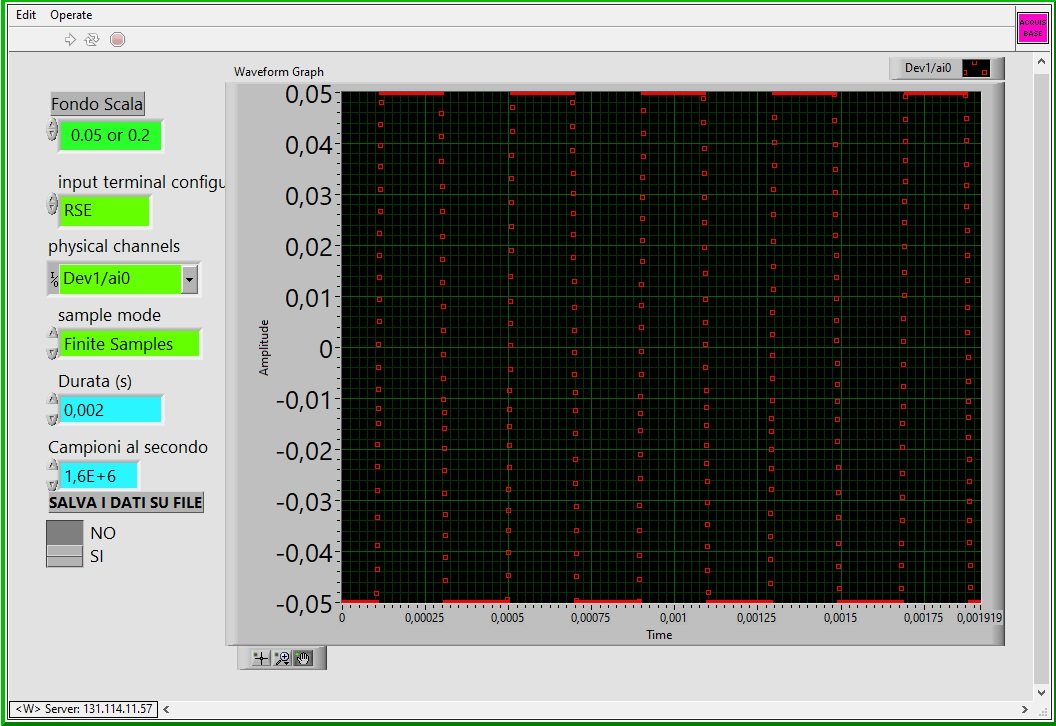
\includegraphics[width=8cm]{settimana_1/immagini/fondoscala.jpg}
    \centering
\end{figure}

\Nota{
    Abbiamo eseguito questa prova come operazione preliminare, tuttavia non abbiamo salvato la schermata in quel momento. L'immagine mostrata si riferisce ad un'acquisizione fatta successivamente. A parte il differente segnale e impostazioni, le stesse osservazioni rimangono valide.
}

\LogMark{Prima acquisizione}{16:09}
Abbiamo fatto alcune prove cambiando fondoscala, tempo di acquisizione e frequenza di campionamento per trovare delle impostazioni che ci permettessero di acquisire correttamente la forma d'onda attualmente in ingresso. Abbiamo scelto le seguenti impostazioni per ottenere la migliore risoluzione sulle letture senza toccare il fondoscala:
\begin{itemize}
    \item $\text{fondo scala} = 0.5 V$
    \item $\text{input terminal configuration} = RSE$
    \item $\text{physical channels} = Dev1/ai0$
    \item $\text{sample mode} = Finite Samples$
    \item $\text{Durata [s]} = 0.0005$
    \item $\text{Campioni al secondo} = 1.6 \cdot 10^6$
\end{itemize}

\begin{figure}[H]
\caption{}
    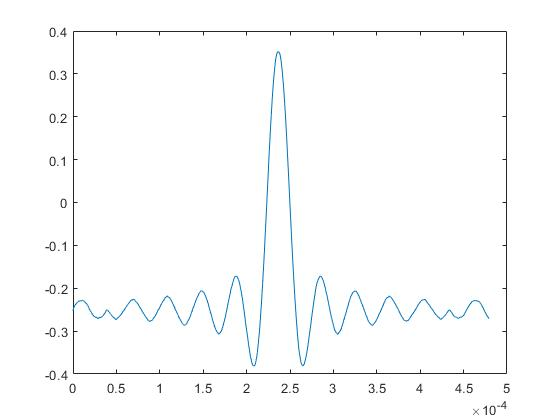
\includegraphics[width=8cm]{settimana_1/immagini/prima_matlab.jpg}
    \centering
\end{figure}

\Nota{
    Sul momento non abbiamo catturato l'immagine della schermata. A titolo esplicativo, abbiamo inserito in un momento successivo il grafico dallo script di analisi Matlab.
}

I dati di questa acquisizione i trovano in \verb+settimana_1/Dati_TD_1/acquisizione1.txt+.

\Nota{
    La frequenza di campionamento massima della nostra scheda è di circa $1.8MS/s$, tuttavia non è possibile acquisire né a $1.8MSa/s$ né a $1.7MSa/s$ (non restituisce misure). Scegliamo allora di usare come frequanza massima $1.6MSa/s$. Sarebbe possibile trovare un valore migliore, ma non è nell'interesse dell'esercizio.
}

\LogMark{Acquisizioni con nuova forma d'onda}{16:13}
Notiamo che la forma d'onda è cambiata. Cerchiamo dei parametri differenti per acquisire con le nuove condizioni:\\
\begin{figure}[H]
\caption{}
    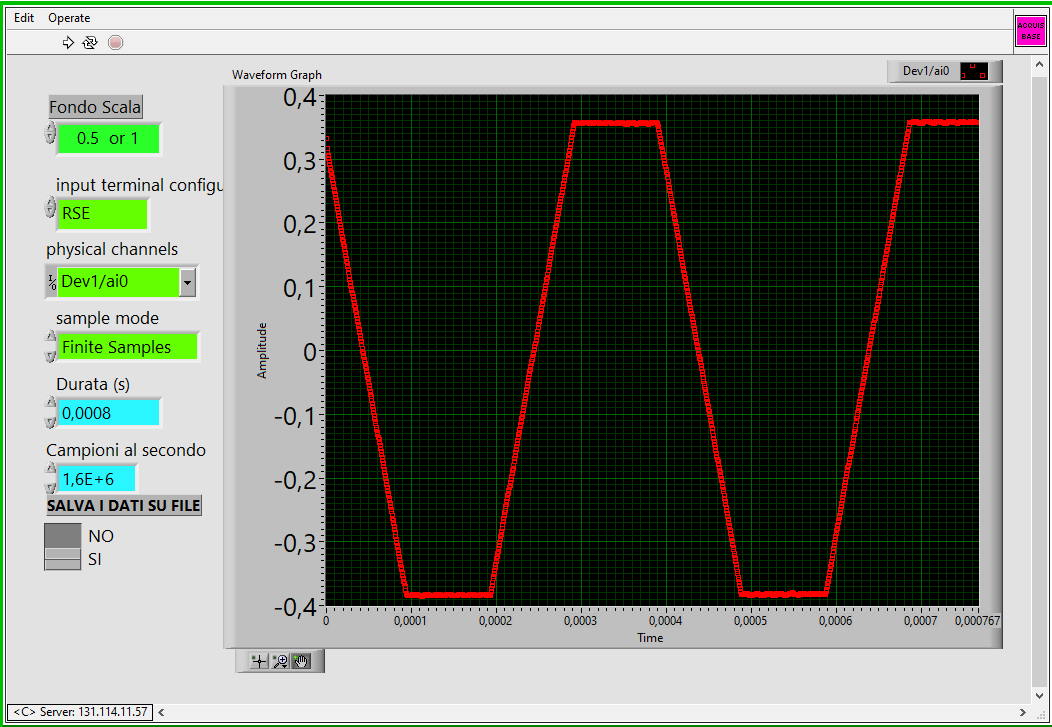
\includegraphics[width=8cm]{settimana_1/immagini/nuova_forma.png}
    \centering\label{Figura:acquis2}
\end{figure}
I dati di questa acquisizione i trovano in \verb+settimana_1/Dati_TD_1/acquisizione2.txt+ e successivi, presi con differenti combinazioni di parametri di acquisizione.

\NewSection{Partitore di tensione (Es. 12)} 
All'interno del presente esercizio, vogliamo fare delle acquizioni su un apparato fisico costituito da un partitore di tensione, con i collegamenti illustrati in figura.
\begin{wrapfigure}{r}{0.3\textwidth}
  \caption{}
    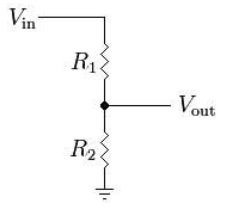
\includegraphics[width=0.3\textwidth]{settimana_1/immagini/partitore.jpg}
\end{wrapfigure}
Ove $V_{in}$ può essere regolata da  attraverso la piattaforma \textcolor{airforceblue}{\url{http://131.114.11.57:8000/ACQUIS.html}}. Il programma acquisisce varie misure di $V_{in}$ e $V_{out}$ e restituisce la media e la deviazione standard. I segnali idealmente sono legati dalla relazione:
\begin{equation}
    V_{out} = V_{in} {1 \over{{R_1\over{R2}} + 1}}
\label{eq1.2}
\end{equation} 
Quindi, supposto (come ragionevole entro certi limiti di temperatura locale) che le resistenze assumano valore costante, avremo un rapporto $V_{out} \over{V_{in}}$ a sua volta costante. Vogliamo verificare queste assunzioni. Per fare tale operazione, abbiamo realizzato due gruppi di acquizioni indipendenti, inerenti a due differenti partitori di tensione:
\begin{itemize}
    \item Primo partitore: la tensione  $V_{in}$ è generata dal canale \textbf{ao0} e viene acquisita attraverso \textbf{ai1}. $V_{out}$ viene rilevata da \textbf{ai2};
    \item Secondo partitore: la tensione  $V_{in}$ è generata dal canale \textbf{ao1} e viene acquisita attraverso \textbf{ai3}. $V_{out}$ viene rilevata da \textbf{ai4};
\end{itemize}

\Nota{
    All'interno delle acquizioni, si tiene conto che la risoluzione della misura varia proporzionalmente al fondo scala fs adottato. Infatti, una volta scelto un fondo scala, il range massimo entro cui puuò evolvere l'acquisizione è pari a $2 \cdot fs$. Il numero di livelli digitali disponibili per l'acquisizione sono pari a $2^{N_{BIT}}$, ove $N_{BIT}$ è la dinamica della scheda. Conseguentemente, la risoluzione della misura è definita attraverso la legge:
    \begin{equation}
        Risoluzione = {{2 fs}\over{2^{N_{BIT}}}} = {fs \over{2^{N_{BIT} - 1}}}
    \end{equation}
    La 6024 fa una lettura con dinamica di profondità 12 bit. Quindi abbiamo $2^{12}= 4096$ livelli.\newline
    Conseguentemente alla diretta proporzionalità fra la risoluzione e fs, è opportuno ai fini di una misura ottimale adottare quale fondo scala il minimo che consenta la copertura dei valori assunti dal segnale sotto studio.
}
\Avvertimento{L'esercizio richiede di effetture delle misure spaziando da -10 V a +10 V. Noi spaziamo solo entro i valori positivi di tensioni (per svista).}

Le misure effettuate per il primo partitore sono riportate di seguito:
\begin{center}
\begin{tabular}{|c|c|c|c|c|c|c|}
\hline
$V_{in}$ [V]          &$fs1 [V]$        &$fs2 [V]$        &$V_{in}$ medio $[V]$        &$V_{in}$ dev.std. $[V]$        &$V_{out}$ medio $[V]$        &$V_{out}$ dev.std. $[V]$\\
\hline
9.00            & 10.00     & 10.00        & 8.98449     & 0.00075        & 4.9368     & 0.0012          \\
7.00         & 10.00     & 10.00        & 6.98741     & 0.00072        & 3.83787     & 0.00083           \\
5.00           & 5.00     & 5.00        & 4.9888     & 0.0012        & 2.7375     & 0.0013           \\
3.00         & 5.00     & 5.00        & 2.98626     & 0.00092        & 1.63710     & 0.0013           \\
1.00          & 5.00     & 5.00        & 0.99112     & 0.00046        & 0.5383     & 0.0013       \\
\hline
\end{tabular}
\end{center}
All'interno della tabella, sono indicati con $fs1$ e $fs2$ i valori di fondoscala adottati per l'acquisizione dei segnali $V_{in}$ e $V_{out}$ rispettivamente.
\Avvertimento{
    Per la secona misura del precedente gruppo di acquisizioni abbiamo usato un fondoscala di $10V$, ma erano sufficienti $5V$ (la misura sarebbe probabilmente risultata più precisa).
}

\Avvertimento{
    I valori medi sono stati calcolati dal nodo \textit{MEAN} di LabVIEW su circa 200 misure (scelta effettuabile attraverso la piattaforma). Non sappiamo se le deviazioni standard si riferiscono alla media o al campione. Abbiamo successimamente letto la documentazione che chiama tale valore "Error", quindi suponiamo si riferisca alla media.
}

\Nota{
    Nelle misure di tensione abbiamo una risoluzione di $2/4096$ del fondo scala, tuttavia nella tabella è riportata la media di una serie di queste. Dunque suponendo che "sd" si riferisca all'errore sulla media, abbiamo scelto il numero di cifre adeguato
}

Le misure effettuate per il secondo partitore sono riportate di seguito:
\begin{center}
\begin{tabular}{|c|c|c|c|c|c|c|}
\hline
$V_{in}$ [V]          &$fs1 [V]$        &$fs2 [V]$        &$V_{in}$ medio $[V]$        &$V_{in}$ dev.std. $[V]$        &$V_{out}$ medio $[V]$        &$V_{out}$ dev.std. $[V]$\\
\hline
9.00           &10.00    &5.00        &8.9918    &0.0024    &1.6005    &0.0015\\
7.00         &10.00    &5.00    &6.99229    &0.00071    &1.2424    &0.0015\\
5.00           &5.00    &5.00     &4.99234    &0.00084    &0.8827    &0.0015\\ 
3.00         &5.00    &5.00    &2.98828    &0.00005    &0.5236    &0.0015\\
1.00         &5.00    &0.5    &0.99116    &0.00034    &0.1656     &0.0013\\
\hline
\end{tabular}
\end{center}

\LogMark{Calcolo ${V_{in}}/{V_{out}}$}{18:10 circa}
Calcoliamo il rapporto $\frac{V_{in}}{V_{out}}$ per la prima acquisizione effettuata con ciascun partitore. I risultati ottenuti sono $1.82$ e $5.57$ (rispettivamente per il primo ed il secondo partitore).

\TODO{
    \sout{Sul posto abbiamo calcolato solo il primo valore per mancanza di tempo, gli altri da fare.} Fatto il 26/09
}

\LogMark{Calcolo ${R_1}/{R_2}$}{18:10 circa}
Per ogni partitore, calcoliamo il rapporto ${R_1}/{R_2}$ sulla base dei dati ottenuti dalla prima acquisizione per ciascun apparato. I risultati sono rispettivamente $0.82$ e $4.57$ (approssimativamente: non forniamo qui una stima dell'errore).

\TODO{
   \sout{Da fare successivamente: calcola gli altri raporti (con le opportune incertezze) e vedi se sono compatibili.} Fatto il 26/09
}

\NewSection{Automazione misure}
Entriamo nel link \textcolor{airforceblue}{\url{http://131.114.11.57:8000/TRACCIA.html}}. Al suo interno vi è una piattaforma che consente il controllo dei partitori previamente adottati. Essa avvia un'acquisizione di N misure delle coppie ($V_{in}$, $V_{out}$), variando linearmente la tensione in ingresso $V_{in}$ fra un valore $V_{min}$ e $V_{max}$, impostabili dall'utente. Anche il numero N può essere scelto attraverso questa piattaforma. Inoltre, vanno selezionati i canali di ingresso e di uscita, analogamente a quanto fatto nella precedente sezione.
Una volta avviata l'acquisizione, appare un grafico ove sono sono rappresentate le coppie $(V_{in} impostata, V_{in} misurata)$ e $(V_{in} impostata, V_{out} misurata)$, contradistinte da due colori diversi (rispettivamente bianco e rosso). Allo stesso tempo, se impostato il salvataggio dell'acquisizione, si genera un file a 3 colonne così nominate: $V_{in}$ impostato (in volt), $V_{in}$ misurato (in volt) e $V_{out}$ misurato (in volt). 

\LogMark{Realizzazione dell'acquisizione di prova (primo partitore)}{18:29}
Impostiamo quale canale di uscita ao0 e quali canali ingresso 1 e 2 rispettivamente ai1 e ai2, così da esaminare il primo partitore. Effettuiamo un'acquisizione di prova con i parametri di default, ai fini di verificare il funzionamento della piattaforma.
Di seguito il grafico corrispondente alla \text{"presa1.txt"}:
\begin{figure}[H]
\caption{}
    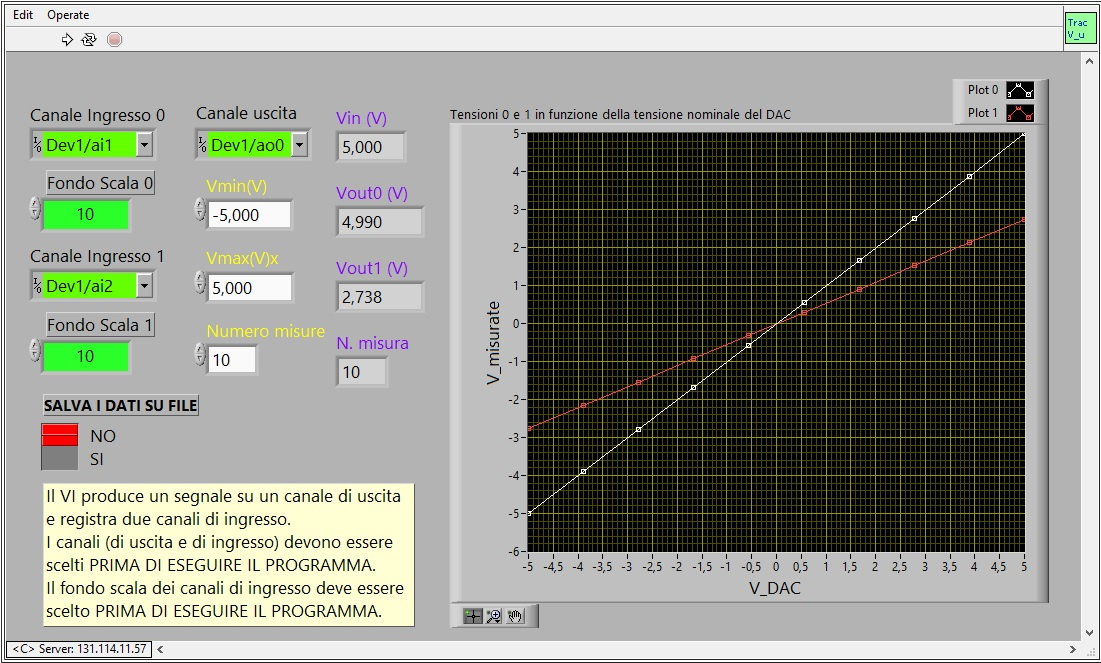
\includegraphics[width=8cm]{settimana_1/immagini/traccia_prova.jpg}
    \centering
\end{figure}
I dati di questa acquisizione si trovano in \verb+settimana_1/partitori_2/presa1.txt+

\LogMark{Acquisizione ottimale (primo partitore)}{18:31}
Ora impostiamo dei parametri ottimali in vista di un'analisi dati successiva. Più precisamente adottiamo: $N = 200$, $V_{max} = fs = - V_{min} = 10 V$. Di seguito il grafico corrispondente al primo partitore:
\begin{figure}[H]
\caption{}
    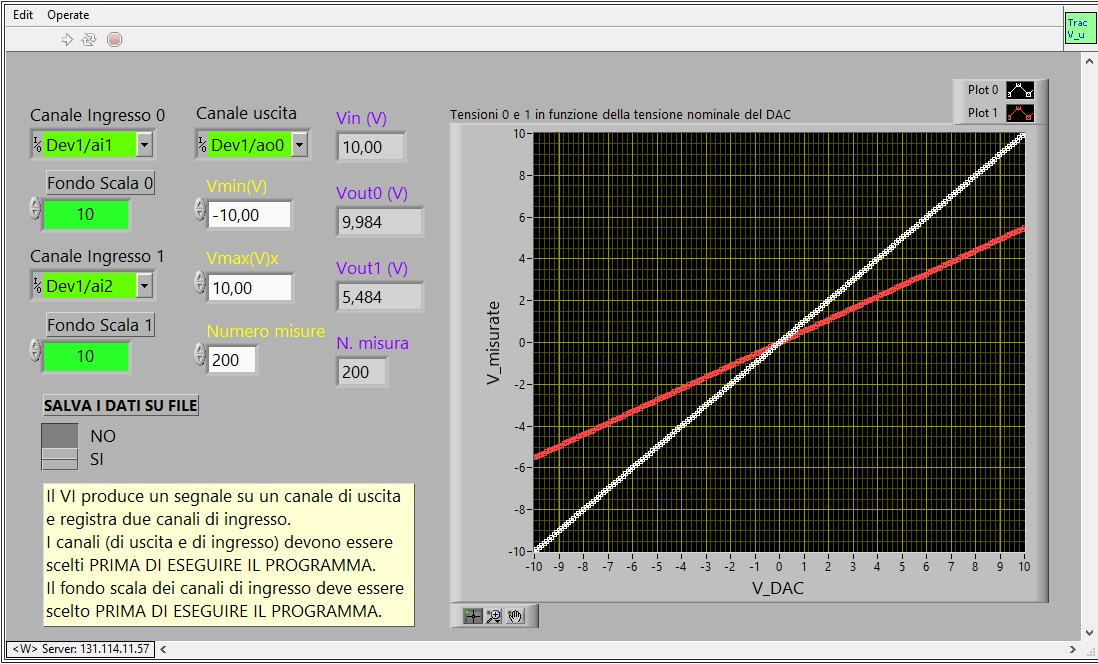
\includegraphics[width=8cm]{settimana_1/immagini/traccia_2.jpg}
    \centering
\end{figure}
I dati di questa acquisizione si trovano in \verb+settimana_1/partitori_2/presa2.txt+

\LogMark{Realizzazione dell'acquisizione di prova (secondo partitore)}{18:32}
Impostiamo quale canale di uscita ao1 e quali canali ingresso 1 e 2 rispettivamente ai3 e ai4, così da esaminare il secondo partitore. Effettuiamo un'acquisizione di prova con i parametri di default della piattaforma, ai fini di verificarne il funzionamento.
Di seguito il grafico corrispondente alla \text{"presa3.txt"}:

\begin{figure}[H]
\caption{}
    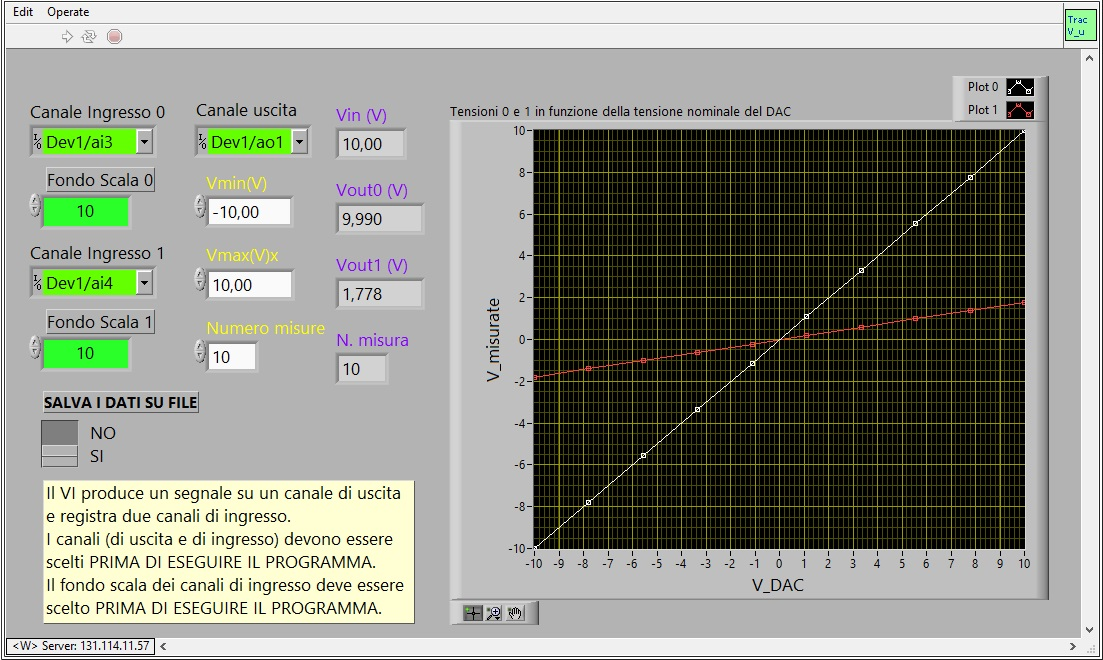
\includegraphics[width=8cm]{settimana_1/immagini/traccia_3.jpg}
    \centering
\end{figure}
I dati di questa acquisizione si trovano in \verb+settimana_1/partitori_2/presa3.txt+
\Nota{
    Per questa acquisizione avremmo potuto usare il fondoscala a $5V$, tuttavia non abbiamo considerato per errore questa possibilità durante l'acquisizione.
}

\LogMark{Acquisizione ottimale (secondo partitore)}{18:37}
Ora impostiamo dei parametri ottimali in vista di un'analisi dati successiva. Più precisamente impostiamo: $N = 200$, $V_{max} = fs = - V_{min} = 10 V$. Di seguito il grafico corrispondente al secondo partitore:
\begin{figure}[H]
\caption{}
    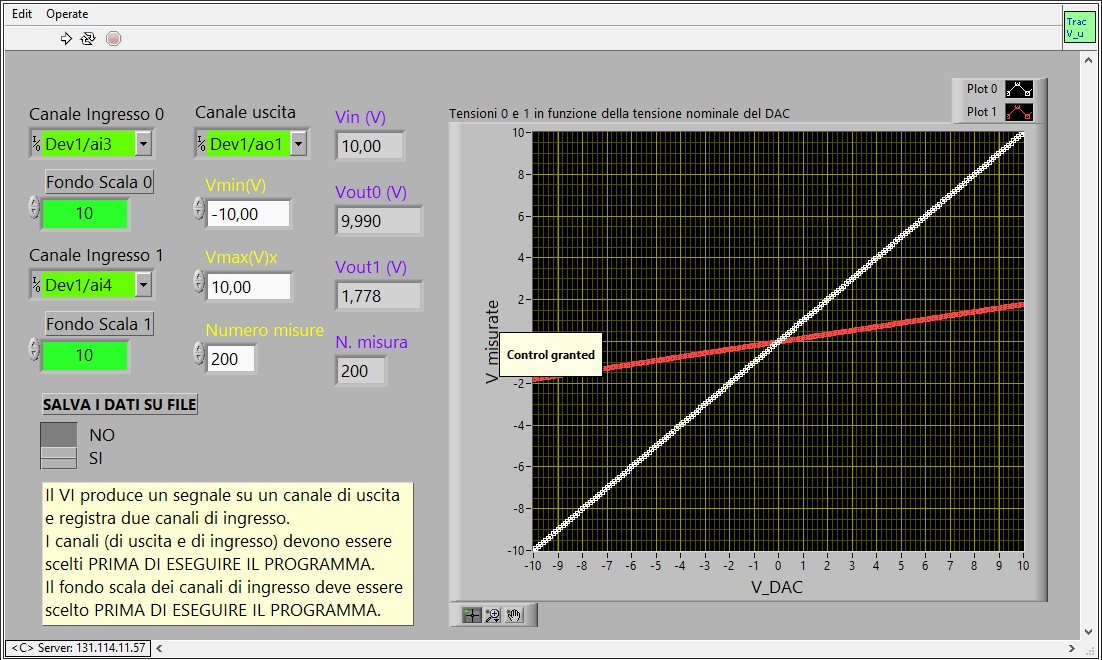
\includegraphics[width=8cm]{settimana_1/immagini/traccia_4.jpg}
    \centering
\end{figure}
I dati di questa acquisizione i trovano in\verb+settimana_1/partitori_2/presa4.txt+



\LogMark{Analisi dati}{18:40 - 18:50}
Analizziamo ora i dati della seconda presa. Effetuiamo un fit degli scarti quadratici lineare delle coppie $(V_{in} misurata, V_{out} misurata)$, ai fini di valutare l'effettiva linearità dell'andamento. 
\Nota{
    L'ambiente di lavoro Matlab non è ancora stato introdotto, pertanto utilizziamo uno script in Python per eseguire l'analisi dei dati.
}
La legge adottata per il fit è:
\begin{equation}
    f(x; a, b) = {x \over{a}} + b
\end{equation}
ove a e b sono parametri liberi.
I risultati del fit sono:
\begin{center}
\begin{verse}
\begin{equation}
    a = 1.81745 \pm 0.00004
\end{equation}\par
\begin{equation}
    b = -0.00753 +- 0.00007
\end{equation}\par
\begin{center}
Absolute sigma = False\par
\end{center}
\end{verse}
\end{center}
Riportiamo di seguito il grafico con i dati e la retta di fit, con sottoposto il relativo grafico dei residui:
\begin{figure}[H]
\caption{}
    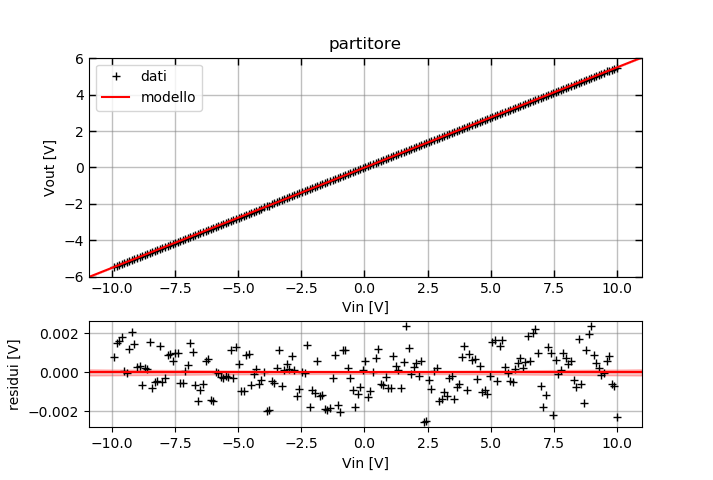
\includegraphics[width=8cm]{settimana_1/immagini/fit_1.png}
    \centering
\end{figure}

Idealmente la stima di b dovrebbe risultare compatibile con zero. Tuttavia per le specifiche tecniche della scheda e per il tipo di calibrazione effettuata, le misure potrebbero essere soggette da un errore di zero. Ciò non è indice di alcuna relazione particolarmente peculiare fra gli andamenti dei due segnali acquisiti.
Il parametro $a$, quindi, rappresenta effettivamente il rapporto $V_{in}/V_{out}$. Conseguentemente, adottando l'equazione \eqref{eq1.2},
il valore $R_{1}/R_{2}$ stimato risulta essere $0.81745 \pm 0.00004$.

Analizziamo ora i dati della quarta presa. Effetuiamo un fit degli scarti quadratici lineare delle coppie $(V_{in} misurata, V_{out} misurata)$, ai fini di valutare l'effettiva linearità dell'andamento. Procedendo analogamente al precedente fit, otteremo i seguenti risultati:
\begin{center}
\begin{verse}
\begin{equation}
    a = 5.5740 \pm 0.0003
\end{equation}\par
\begin{equation}
    b = -0.01339 \pm 0.00006
\end{equation}\par
\begin{center}
Absolute sigma = False\par
\end{center}
\end{verse}
\end{center}

Riportiamo di seguito il grafico con i dati e la retta di fit, con sottoposto il relativo grafico dei residui:
\begin{figure}[H]
\caption{}
    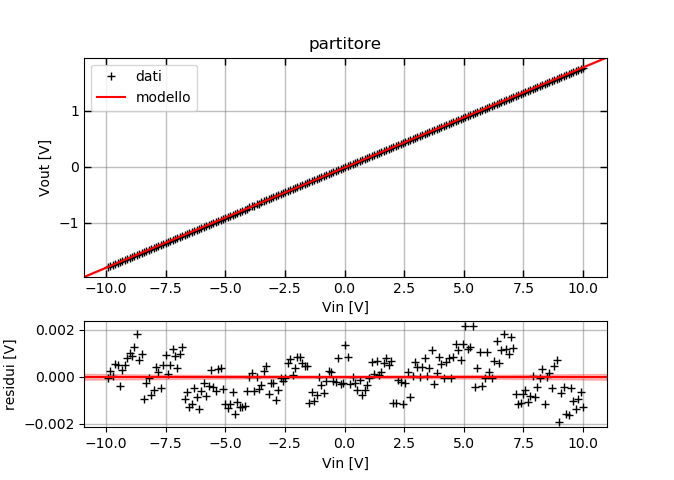
\includegraphics[width=8cm]{settimana_1/immagini/fit_2.png}
    \centering
\end{figure}

Valgono le stesse condiserazione effettuate per la seconda presa. Il valore $R_{1}/R_{2}$ stimato risulta essere $4.5740 \pm 0.0003$.

\Nota{
    Nelle procedure di fit, scegliamo di ulitizzare \textit{absolute sigma = False} (cioè l'incertezza sui parametri trovati viene rinormalizzata in base al valore del $S^2$ ridotto). Questo perchè non conosciamo la reale incertezza sulle misure. Scegliamo, inoltre, di assegnare pesi uguali a tutti i punti.
}

\Nota{
    Poichè non conosciamo l'incertezza delle misure, risulta azzardato trarre conclusioni circa la compatibitità dei dati con la legge lineare.
}

\LogMark{Acquisizione con maggiore numero di punti (secondo partitore)}{18:57}
Nel tempo rimasto acquisiamo un maggior numero di punti per il secondo pertitore (1000 misure). Il nostro obiettivo è quello di capire se l'andamento delle coppie $V_{out} \: vs \: V_{in}$ sia effettivamente lineare.
Eseguiamo l'analisi precedente per il nuovo set. Il grafico risulta il seguente:
\begin{figure}[H]
\caption{}
    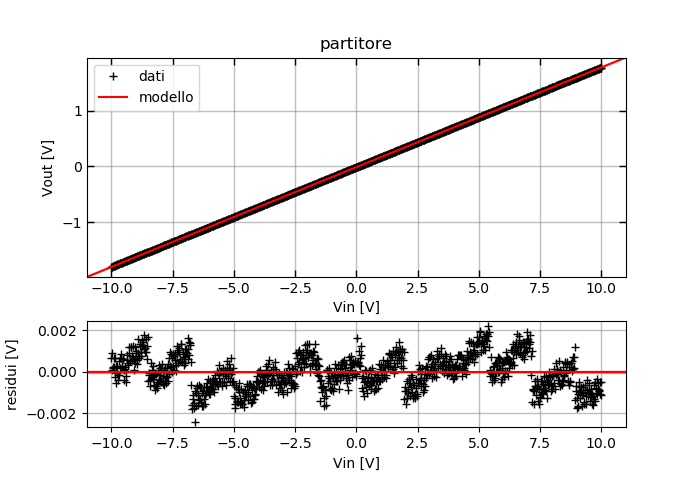
\includegraphics[width=8cm]{settimana_1/immagini/Figure_5.png}
    \centering
\end{figure}

Come negli altri grafici, notiamo un andamento "a S" dei residui. Tuttavia è presente una sorta di conformazione "a gradini". Ciò è in parte dovuto alla scelta erronea della scala da $10V$ per $V_{out}$. Considerando inoltre che la risoluzione è $0.005V$, l'effetto della discretizzazione delle misure può anch'essa dar luogo a tale andamento dei residui.


\NewDay{Alcune attività successive}{26/09/2020}
\NewSection{Ulteriore analisi sulle misure della sezione Partitore di tensione (Es. 12) (del giorno 24/09/2020)}
\Orario{12:00-12:50}

Per ogni acquisizione col primo partitore, calcoliamo il rapporto $V_{out}/{V_{in}}$:
\begin{center}
\begin{tabular}{|c|c|c|c|c|c|c|}
\hline
$V_{in} [V]$          & $ {V_{out}/V_{in}}$ \\
\hline 
9.00         &    $1.8199 \pm 0.0003$   \\
7.00         &    $1.8206 \pm 0.0003$   \\
5.00         &    $1.8224 \pm 0.0006$   \\
3.00         &    $1.8241 \pm 0.0009$   \\
1.00         &    $1.841 \pm 0.003$   \\
\hline
\end{tabular}
\end{center}
Osserviamo che i valori ottenuti \textcolor{red}{non} risultano essere compatibili entro l'incertezza per i vari valori di $V_{in}$. Questo si può spiegare considerando che abbiamo utilizzato come incertezze le varianze della media. Tuttavia in tal modo stiamo considerando solo l'errore statistico, mentre non si tiene in conto di quello di origine sistematica (ad esempio la non linearità degli ADC ed eventualmente gli assorbimenti di questi).

Sulla base degli stessi è possibile calcolare il rapporto ${R_1}/{R_2}$ per il primo partitore:
\begin{center}
\begin{tabular}{|c|c|c|c|c|c|c|}
\hline
$V_{in} [V]$          & $ {R_1/R_2}$ \\
\hline 
9.00         &    $0.8199 \pm 0.0003$   \\
7.00         &    $0.8206 \pm 0.0003$   \\
5.00         &    $0.8224 \pm 0.0006$   \\
3.00         &    $0.8241 \pm 0.0009$   \\
1.00         &    $0.841 \pm 0.003$   \\
\hline
\end{tabular}
\end{center}
Osserviamo che i valori ottenuti \textcolor{red}{non} risultano essere compatibili entro l'incertezza per i vari valori di $V_{in}$ (per i motivi sopra elencati).

Successivamente, per ogni acquisizione col secondo partitore, calcoliamo il rapporto $V_{out}/V_{in}$:
\begin{center}
\begin{tabular}{|c|c|c|c|c|c|c|}
\hline
$V_{in} [V]$          & $ {V_{out}/V_{in}}$ \\
\hline 
9.00         &    $5.618 \pm 0.003$   \\
7.00         &    $5.628 \pm 0.003$   \\
5.00         &    $5.656 \pm 0.005$   \\
3.00         &    $5.707 \pm 0.008$   \\
1.00         &    $5.98  \pm 0.03$    \\
\hline
\end{tabular}
\end{center}
Osserviamo che i valori ottenuti \textcolor{red}{non} risultano essere compatibili entro l'incertezza per i vari valori di $V_{in}$ (vedi osservazioni per il partitore precedente).
Sulla base degli stessi è possibile calcolare il rapporto ${R_1}\over{R_2}$ per il secondo partitore:
\begin{center}
\begin{tabular}{|c|c|c|c|c|c|c|}
\hline
$V_{in} [V]$          & $ {R_1}/{R_2}$ \\
\hline 
9.00         &    $5.618 \pm 0.003$   \\
7.00         &    $5.628 \pm 0.003$   \\
5.00         &    $5.656 \pm 0.005$   \\
3.00         &    $5.707 \pm 0.008$   \\
1.00         &    $5.98  \pm 0.03$    \\
\hline
\end{tabular}
\end{center}
Osserviamo che i valori \textcolor{red}{non} ottenuti risultano essere compatibili entro l'incertezza per i vari valori di $V_{in}$(vedi osservazioni per il partitore precedente).

\NewSection{Analisi dati con Matlab (dati da \text{"Acquisizione forme d'onda"} del 24/09/2020) (Hw. 1)}
Realizziamo\Orario{16:06-17:00}uno scipt in Matlab per visualizzare, determinare il minimo e il massimo di una delle acquisizioni (più precisamente in \verb+"acquisizione3.txt"+). All'interno dello stesso, inoltre, effettuiamo un fit con una sinusoidale, ai fini di determinare il periodo della forma d'onda sotto studio (trovandone l'armonica principale).
Lo scipt usato:

\begin{verbatim}
[x, y] = leg_wavf("acquisizione3.txt");
plot(x, y);
fprintf("massimo = %f\n", max(y));
fprintf("minimo = %f\n", min(y));

f = @(a, b, c, om, x) a * sin(x * om + c) + b;
fitfun = fittype(f);
X0 = [0.35, 0, 2, 1.5 * 10^4];
[fitted_curve, gof] = fit(x, y, fitfun, "StartPoint", X0);
coeffvals = coeffvalues(fitted_curve);
fprintf("periodo = %f\n", 2 * pi / coeffvals(4));
scatter(x, y, "+")
hold on;
plot(x, f(coeffvals(1), coeffvals(2), coeffvals(3), coeffvals(4), x))
hold off;
\end{verbatim}

I risultati conseguiti risultano essere:
\begin{align*}
\flushleft
	massimo &\approx 0.3694 V \\
	minimo &\approx -0.3851 V \\
	periodo &\approx 0.000395 s\\
\end{align*}

\Nota{
    Abbiamo usato un'acqusizione di una forna d'onda trapezioidale. Sarebbe stato possibile farlo anche per la prima forma d'onda, tuttavia l'intervallo che abbiamo acquisito risulta troppo piccolo, dunque eseguire un fit con una forma sinusoidale avrebbe avuto scarso significato.
}
\Nota{Essendo il fondo scala adottato pari a 0.5 V, allora la risoluzione risulta essere $240 \mu V$}

Il grafico della forma d'onda acquisita e della sinuoide principale ottenuta dal fit è il seguente:
\begin{figure}[H]
\caption{}
    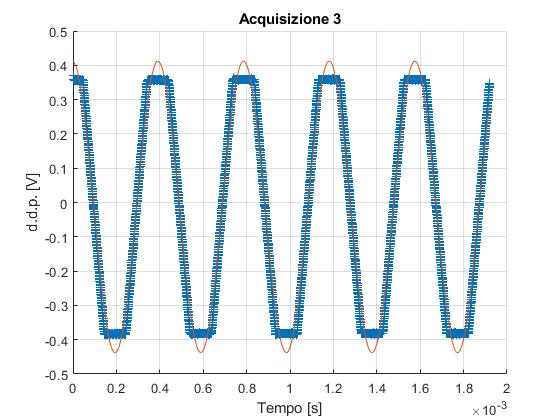
\includegraphics[width=8cm]{settimana_1/immagini/matlab_acquis3.jpg}
    \centering
\end{figure}

\NewSection{Creazione di OUTPUT BASE (Es. 10)}
\LogMark{Cambi tipo I/O}{21:59} 
Vogliamo realizzare un VI capace di comandare una scheda di acquisizone a generare una tensione. La struttura di base dello schema nel "Block Diagram" risulterà simile a quella per l'acquisione di segnali esterni. Quindi, riprendendo il diagramma \ref{figura:diagramma}, è sufficiente fare le seguenti modifiche:
\begin{itemize}
    \item modificare \textit{AI voltage} in \textit{AO voltage}. Tramite questa sola operazione, inoltre, il canale fisico di input e l'input terminal configuration divengono automaticamente rispettivamente il canale fisico di output e l'output terminal configuration;
    \item al timing scolleghiamo tutto tranne il rate, che però modifichiamo a costante predefinita, e il sample mode;
    \item al source del timing colleghiamo un  controllo;
    \item al posto del read, inseriamo un write.
    \item facciamo i seguenti collegamenti col write:
    \begin{itemize}
        \item al task in colleghiamo il task out del timing;
        \item al task out colleghiamo uno stop;
        \item all'auto start colleghiamo una costante booleana;
        \item al data colleghiamo un controllo, che chiamiamo $V_{in}$ (volt).
    \end{itemize}
\end{itemize}
Di seguito riporto il diagramma realizzato:
\begin{figure}[H]
\caption{}
    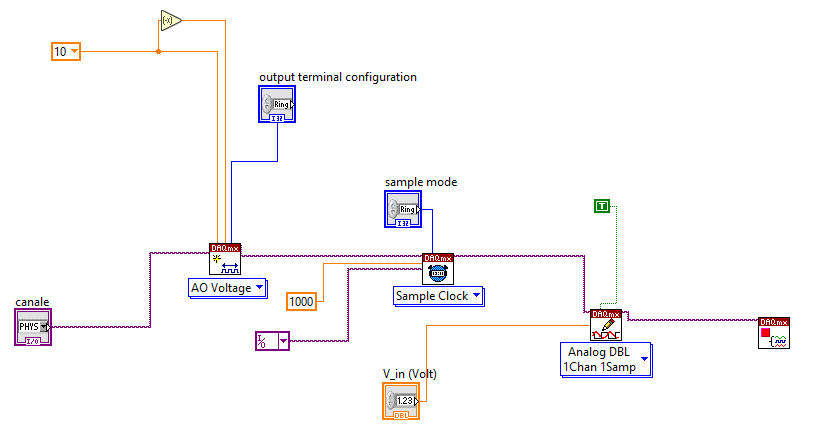
\includegraphics[width=8cm]{settimana_1/immagini/MXVOUT.png}
    \centering
\end{figure}

\Nota{
    A differenza del diagramma \ref{figura:diagramma}, poniamo costanti il sample rate e la durata. Infatti, dato che utilizzeremo questo VI per generare tensioni fisse, modificare tali impostazioni non avrebbe alcun effetto.
}

\NewSection{Creazione di VinVout (Es. 11)}
\Orario{23:00}
Vogliamo realizzare un VI che permetta di generare una tensione impostata e leggere un segnale analogico dopo un tempo prestabilito, visualizzandolo e facendone la media.
Partiamo da un VI Vuoto. Inseriamo una sequenza di 3 frame, in cui immettiamo:
\begin{enumerate}
  \item il diagramma di OUTPUT BASE;
  \item una pausa controllabile dal Pannello;
  \item il diagramma per la lettura analogica.
\end{enumerate}

Nell'ultimo frame, all'output della lettura colleghiamo il nodo \textit{"Convert from Dynamic Data"}. Questo permette di accumulare i dati, generati dinamicamente, in un array. Attravero l'operazione \text{Mean}, calcoliamo la media e la corrispondente deviazione standard sugli elementi dell'array. Visualizziamo tali valori in due \text{"Numeric indicator"}.
I 3 frame realizzati sono riportati nelle figure seguenti:
\begin{figure}[H]
\caption{frame per la generazione del segnale}
    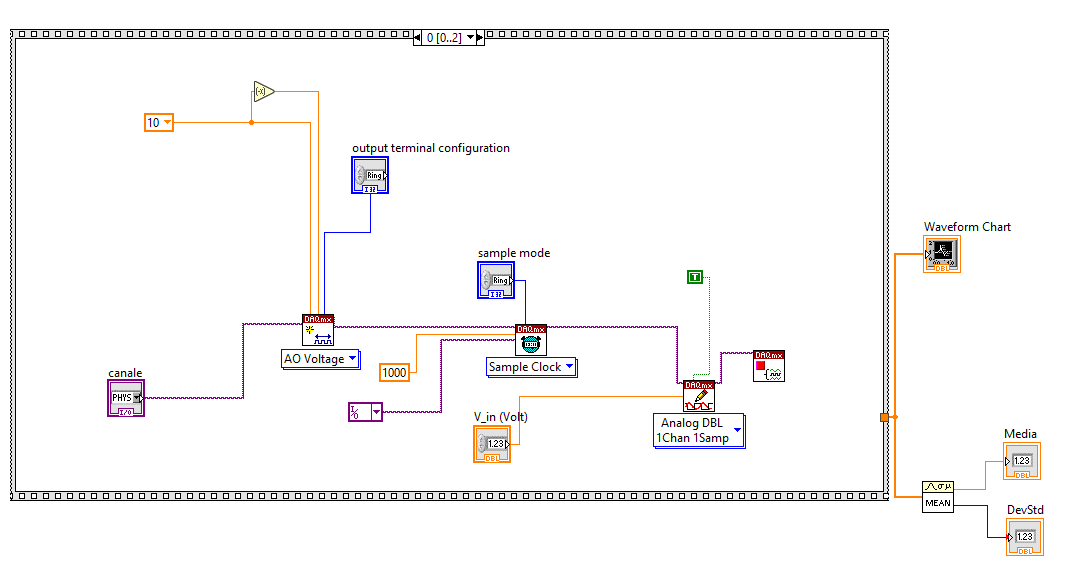
\includegraphics[width=10cm]{settimana_1/immagini/MXVinVout0su2.png}
    \centering
\end{figure}
\begin{figure}[H]
\caption{frame per l'attesa impostata}
    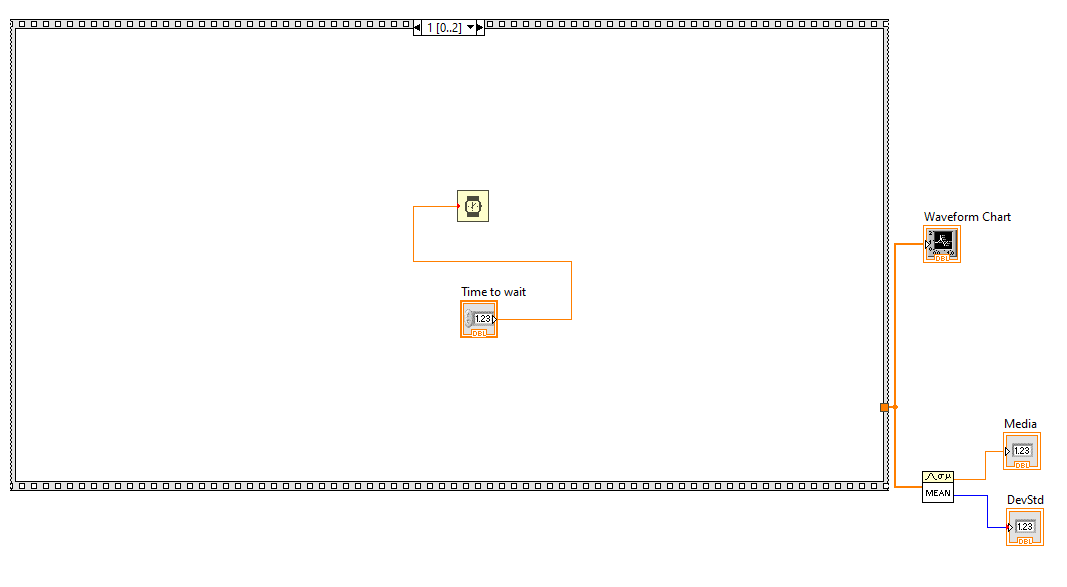
\includegraphics[width=10cm]{settimana_1/immagini/MXVinVout1su2.png}
    \centering
\end{figure}
\begin{figure}[H]
\caption{frame per la lettura analogica}
    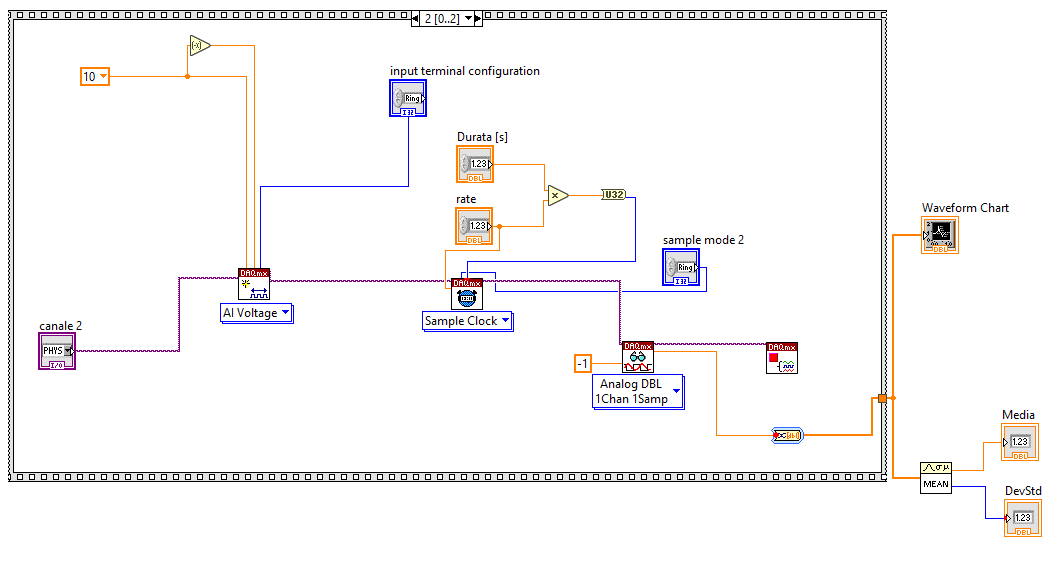
\includegraphics[width=10cm]{settimana_1/immagini/MXVinVout2su2.png}
    \centering
\end{figure}